\documentclass[a4paper,12pt]{article}

%benötigte Pakete
\usepackage[ngerman]{babel}		%Deutscher Standard
\usepackage[T1]{fontenc}			%Ausgabefont
\usepackage[utf8]{inputenc}		%Umlaute
\usepackage{amsmath}				%Formeln einbinden
\usepackage{mathptmx}			%Schriftart Times
\usepackage{graphicx}			%Paket für Grafiken
\usepackage{hyperref}			%Verlinkungen
\usepackage{float}
\usepackage[bottom]{footmisc}	%Fußnote am Ende der Seite darstellen

%Literaturangaben
\bibliographystyle{unsrt}

%Sonstiges
\setlength\headheight{40pt}
%\setlength\footskip{50pt}
%\setlength{\topmargin}{1cm}
\usepackage[left=3cm,right=3cm,top=2cm,bottom=2cm,includeheadfoot]{geometry}
\title{Entwicklerdokumentation M5Stick Überwachungssystem}
%\date{\today} %aktuelles Datum einfügen
\graphicspath{{Bilder/}} %Bilderpfad 

%Kopf- und Fußzeile erstellen
\usepackage{fancyhdr}
\pagestyle{fancy}
\lhead{\includegraphics[height=1.2cm]{Allgemeines_Logo.jpg}}
%\lhead{\thesubsection}
%\chead{Überwachungssystem M5 Stick} %Mitte Kopfzeile
\rhead{\leftmark}
\lfoot{}
\cfoot{}
\rfoot{\thepage}
%\renewcommand{\headrulewidth}{10pt}	%Dicke der Linie

%Bestelllinks:
%------------------------------------Links-----------------------------------------------------------------------%
\newcommand{\linkPi}{https://www.reichelt.de/raspberry-pi-3-b-4x-1-4-ghz-1-gb-ram-wlan-bt-raspberry-pi-3b--p217696.html}

\newcommand{\linkPiNT}{https://www.reichelt.de/sg/de/raspberry-pi-netzteil-5-v-2-5-a-micro-usb-schwarz-rasp-nt-25-sw-e-p240934.html}

\newcommand{\linkMstick}{https://eckstein-shop.de/M5StackM5StickCPLUSESP32-PICOMiniIoTDevelopmentKit2CInfrared2FRTC2FMic2FLED2FIMU2FPMU}

\newcommand{\linkBuzzer}{https://www.reichelt.de/sg/de/entwicklerboards-summer-aktiv-debo-buzzer-a2-p282660.html}

\newcommand{\linkLankabel}{https://www.reichelt.de/sg/de/cat-6-slim-light-kabel-u-utp-1-5-m-grau-slim-ul6-1-5-gr-p205582.html}

\newcommand{\linkmicrosd}{https://www.reichelt.de/sg/de/microsdhc-speicherkarte-16gb-transcend-class-10-uhs-i-ts16gusdcu1-p220722.html}

\newcommand{\linkTaster}{https://www.reichelt.de/sg/de/entwicklerboards-2-tasten-modul-debo-button2-p316186.html}

\newcommand{\linkJumpercable}{https://www.reichelt.de/sg/de/entwicklerboards-steckbrueckenkabel-40-pole-f-f-20-cm-debo-kabelset12-p282700.html}

%%%
%Befehle:
%\\ Zeilenumbruch, eher vermeiden
%\par oder \\[0,5cm] neuer Absatz
%\newpage Neue Seite
%\pagebreak Neue Seite, vorheriger Text wird bündig abgeschlossen
%\textbf{xxxxx} Fettschrift 
%\underline{xxxxx} Unterstreichen
%\section{Einführung} Neues Kapitel erstellen
%\subsection{xxxxx} Neues Unterkapitel
%\ref{xxxxx} Referenz erstellen
%%%

%Bilderpfad: C:/Users/lukas/Desktop/AutoTech/Bilder/

\begin{document}

%Titelseite erstellen
\begin{titlepage}
	\centering
	\includegraphics[width=5cm]{M5stick-c-1.jpg}\par\vspace{1cm}
	{\scshape\LARGE Hochschule Emden/Leer \par}
	\vspace{1cm}
	{\scshape\Large Projekt Automatisierungstechnik\par}
	\vspace{1.5cm}
	{\huge\bfseries Entwicklerdokumentation: Überwachungssystem basierend
	auf der IMU des
	M5-Sticks\par}
	\vspace{2cm}
	{\Large\itshape Autoren:\par {Lukas Ohdens, 7013982\par
	Michel Grüther, 7013909\par Luca Schulte, 7014030\par Alexander
	Maul, 7014104\par Hauke Helms, 7013828}\par}
	\vfill
	Betreuender Professor\par
	Prof. Dr. Wings

	\vfill

	{\large Emden, \today\par}
\end{titlepage}

%Inhaltsverzeichnis
\tableofcontents
\newpage

\section{Projektbeschreibung}
\subsection{Aufgabenstellung und Konzept}
Unsere Aufgabe besteht darin, ein “Überwachungssystem basierend auf der IMU des M5-Sticks” zu erstellen. Das Überwachungssystem wird als Alarmanlage in einer “Internet of Things” (IoT) Anwendung in einem Smarthome eingebunden. Der M5StickC wird an Türen und Fenstern montiert und fungiert als Sensor, der mithilfe seiner IMU Bewegungen erkennt. Sobald Bewegungen erkannt werden, wird ein Signal ins Netzwerk abgegeben. Ein Raspberry Pi 3B+ (im folgenden Pi), welcher ebenfalls im Netzwerk eingebunden ist, wird die Aufgabe des Brokers übernehmen. Gleichzeitig wird der Pi auch als Subscriber arbeiten. Als Broker gibt der Pi das Signal weiter und verarbeitet es als Subscriber. Der Pi bewertet nun, ob ein Alarm ausgelöst werden soll oder nicht. Es kann beispielsweise ein Zeitfenster eingestellt werden, in dem immer ein Alarm ausgelöst wird - das macht nachts Sinn, oder während der Arbeitszeit. Zusätzlich soll es die Option geben den Alarm manuell am Pi einzuschalten. Wird ein Alarm ausgelöst, ertönt am Pi ein Buzzer, der als Alarmanlage fungiert und die LED im M5StickC leuchtet dauerhaft, um erkennbar zu machen, wo der Alarm ausgelöst wurde. Um den Alarm zu deaktivieren, wird am Pi ein Knopf gedrückt.

\subsection{Herausforderungen}
Zu den Herausforderungen zählen wir zunächst die Einbindung des Raspberry Pi sowie des M5-Sticks in das Netzwerk. Insbesondere der M5StickC kann aufgrund der fehlenden Benutzeroberfläche und den geringeren Anschlussmöglichkeiten für Peripheriegeräte zu Problemen führen.\par
Außerdem sehen wir die Verbindung zwischen Pi und M5StickC innerhalb des Netzwerkes als Herausforderung, da die Geräte mithilfe deren Netzwerkadressen kommunizieren müssen.\par 
Eine weitere Schwierigkeit ist die Einstellung der Empfindlichkeit der 6-Achsen-IMU. Da bereits kleinste Beschleunigungen zu einer Ausgabe führen, könnte der Alarm bereits bei kleinsten Bewegungen durch bspw. Wind ausgelöst werden.\par 
Da der M5StickC eine Einsatztemperatur von 0...60°C abdeckt, sollte das bei der Montage an der Fensterscheibe berücksichtigt werden, da durch erhöhte Sonneneinstrahlung die Rückseite des M5StickC stark aufgeheizt werden kann. 

\subsection{Problemlösungen}
Die Einbindung des Raspberry Pi und M5StickC ins Netzwerk können wir aktuell noch nicht einschätzen und haben dafür auch noch keine Lösungen.\par 
Die Einstellung der Empfindlichkeit der IMU können wir durch Versuche herausfinden. Hier können wir Messungen durchführen, ab wann eine Türöffnung stattfindet oder es sich lediglich um eine schwingende Tür handelt (ausgelöst durch Wind o.Ä.).\par 
Sollte sich aufgrund auf der Temperatur am M5StickC ein Fehlverhalten feststellen lassen müssen konstruktive Maßnahmen ergriffen werden.

\section{Beschreibung der Hardware}
\subsection{Materialliste}
Anmerkung: Die Versandkosten betragen bei Reichelt 5,95€ und bei Eckstein abhängig von der Versandart 1,99€ (nicht verfolgbar, nicht versichert) oder 3,50€ (verfolgbar, versichert).\par Die Versanddauer, die Verfügbarkeit sowie der Kaufpreis können sich aufgrund aktueller Begebenheiten innerhalb kurzer Zeit ändern. Es fällt kein Mindermengenzuschlag an.\par 
%Es gibt eine Vergünstigung für Hochschulen, dazu oben neben der Sprache den Reiter auf Schule, Hochschule, Universität stellen.\\ 
Alle Internetlinks und Preise wurden am 20.04.2022 zuletzt abgerufen. Der aktuelle Gesamtpreis der Bestellung liegt bei 100,80€ zzgl. Versandkosten.

\vspace{1cm}
%\centering

\begin{table}[H]
	\centering
	
	\resizebox{420pt}{!}{
	\begin{tabular}{||p{0,8cm}|p{2,5cm}|p{2,7cm}|l|p{2,0cm}|r|}
		\hline
		Anz. & Bezeichnung               & Artikel-Nr.       	& Einzelpreis   & Bem.					& Bestellink 						  \\ 
		\hline
		\hline
		1      & Raspberry Pi 3B+          & RASPBERRYPI 3 B+ 	& 46,20 € &                           		&\href{\linkPi}{reichelt.de}    	                             \\
		\hline
		1      & Raspberry Pi - Netzteil   & RASP NT 25 SW E      & 7,25 €  &         	               		&\href{\linkPiNT}{reichelt.de}  	                             \\
		\hline
		1      & M5StickC                  &                   	& 29,95€        & Nur M5 Stick C+ verfügbar        &\href{\linkMstick}{eckstein-shop.de} 	                             \\
		\hline
		1      & Ethernet Kabel            & SLIM UL6 1,5 GR 	& 4,10€        & Auch anderes Kabel in Ordnung, wenn bereits bestellt und lagernd            					&\href{\linkLankabel}{reichelt.de}           		 				                           \\
		\hline
		1      & Piezo Buzzer              & DEBO BUZZER A2     	& 1,45 €  		&             					&\href{\linkBuzzer }{reichelt.de}                                \\
		\hline
		1      & Micro SD Karte 16Gb       &  TS16GUSDCU1       &7,95€         &      					& \href{\linkmicrosd}{reichelt.de} \\ 
		\hline
			1      & Taster              &DEBO BUTTON2         &2,20€         &     					&\href{\linkTaster}{reichelt.de}  \\ 
		\hline
		1      & Jumperkabel set              &DEBO KABELSET12        &1,70€         &     					&\href{\linkJumpercable}{reichelt.de}  \\ 
		\hline
		          						                  
	\end{tabular}
}

\caption{Materialliste für das Projekt Überwachungssystem basierend auf der IMU des M5StickC}	
\end{table}

\newpage

\subsection{M5StickC}
\subsubsection{Aufbau des M5StickC}
Der M5StickC ist in einem Kunststoffgehäuse (PC - Polycarbonate) untergebracht. Der Stick verfügt über zwei Taster, die je nach Anwendung frei programmiert werden können. Der Taster A, der in der Abbildung \ref{AufbauM5StickC} zu sehen ist, befindet sich auf der rechten langen Seite und der Taster B auf der Frontseite. Des Weiteren hat der M5Stick ein farbiges Display mit einer Auflösung von 80x160 Pixel bzw. 0,96“ Bildschirmdiagonale. Auf der linken langen Seite befindet sich die AN / AUS / Restart-Taste. Hierüber wird der M5StickC bei zweisekündiger Betätigung ein- und bei sechssekündiger Betätigung ausgeschaltet.  An den beiden kurzen Seiten sind die Schnittstellen (USB-Typ-C, Grove) sowie eine im Raster von 2,54 mm, 8 polige Buchsenleiste für Jumperkabel verbaut. Grove ist ein benutzerfreundliches System, mit dem sich ein Prozessor (z. B. Arduino) mit einer Vielzahl von Modulen, Sensoren und Eingängen verbinden lässt. Auf der Rückseite wird die Pinbelegung der Buchsenleiste dargestellt. \footnote{\cite{M5STACK.}}

\begin{figure}[H]	%[H] um an dieser Stelle anzuzeigen
\begin{center}
\includegraphics[width=10cm]{AufbauM5StickC.jpg}
\caption{Aufbau des Entwicklungsboardes „M5StickC" \protect\cite{M5STACK.}}
\label{AufbauM5StickC}
\end{center}
\end{figure}

\newpage

\subsubsection{Technische Daten des M5StickC}
\begin{itemize}
\item Eingebauter Mikrocontroller ESP 32 mit 240 MHz Dual-Core, 600 DMIPS, 520 KB SRAM
\item Flash Speicher von 4 MB
\item Akku – 95 mAh mit 3,7 V
\item Einsatztemperatur von 0...60 °C
\item Infrarot Übertragung
\item Abmaße (L x B x H) – 48,2 mm x 25,5 mm x 13,7 mm
\item 5 V Ein- und Ausgangsspannung
\end{itemize}

%IMUAchsen
\subsubsection{Verbaute Sensoren}
In dem M5StickC ist ein digitales Mikrofon (SPM1423) und eine Echtzeituhr (BM8563), auch RTC
(Real-Time-Clock) genannt, verbaut. Des Weiteren hat der Stick eine 6-Achsen-IMU (MPU-6886)
verbaut \footnote{\cite{M5STACK.}}. Die Abkürzung IMU steht für „Inertial Measurement Unit“, zu Deutsch
„Inertiale Messeinheit“. Die IMU ist eine Messeinheit, die aus der Kombination aus einem 3-Achsen-Beschleunigungssensors und einem 3-Achsen-Gyroskopsensors besteht. Die Beschleunigung
wird in der X, Y und Z-Richtung gemessen (s. Abb. \ref{IMUAchsen}). Für jede Achse wird eine separate Prüfmasse
verwendet, die bei Beschleunigung oder Verzögerung einen Weg zurücklegt. Der Abstand, der sich aus
dem Weg nach der Beschleunigung minus dem Weg vor der Beschleunigung ergibt, bestimmt die
Kapazität. Die Kapazität wird anschließend von einem Aufnehmer erkannt, in einen Messwert
umgerechnet und als Spannungssignal ausgegeben. Der Endwert des Ausgangs kann auf ±2g, ±4g,
±8g oder ±16g programmiert werden. \footnote{\cite{InvenSense.}}

Bei dem Gyroskop wird zunächst die Drehung um die dazugehörige Achse (s. Abb. \ref{IMUAchsen}) gemessen.
Wenn die Kreisel des Gyroskops um eine Achse gedreht werden, verursacht der Coriolis-Effekt eine
Schwingung, die anschließend von einem kapazitiven Aufnehmer erkannt wird. Das aufgenommene
Signal wird darauf verstärkt und gefiltert, um eine Spannung zu erzeugen. Diese Spannung ist
proportional zu der Winkelgeschwindigkeit des Gyroskops. Die Winkelgeschwindigkeit lässt sich
digital auf ±250, ± 500, ± 1000 oder ±2000 °
s
(dps=degrees per second) programmieren. \footnote{\cite{InvenSense.}}

\begin{figure}[H]	%[H] um an dieser Stelle anzuzeigen
\begin{center}
\includegraphics[width=10cm]{IMUAchsen.jpg}
\caption{Beschleunigungs- und Drehachsen der IMU
\protect\cite{InvenSense.}}
\label{IMUAchsen}
\end{center}
\end{figure}

\newpage

\subsection{Raspberry Pi 3B+}
Der Raspberry Pi ist ein opensource Minicomputer, welcher ursprünglich als kostengünstiges System für Lernzwecke im Bereich der Programmierung gedacht war. \footnote{\cite{RaspberryPi.20.08.2015}} \par
Besonders in der Makerszene erfreut sich der Raspberry Pi (Abb. \ref{pi_mitgehaeuse}) einer großen Beliebtheit. Es sind Projekte vom Desktopcomputer \footnote{\cite{RaspberryPi.20.08.2015}} bis hin zur Steuerung und Überwachung heimischer 3D-Drucker \footnote{\cite{Hauge.20.04.2022}} realisierbar.\\[3mm]
%Das Produktprotfolio reicht vom leistungsschwächeren Raspberry Pi (1Ghz singlecore, 512 MB RAM) zum leistungsstärkeren Raspberry Pi 
%\\[3mm]

	\begin{figure}[H]
	\centering
	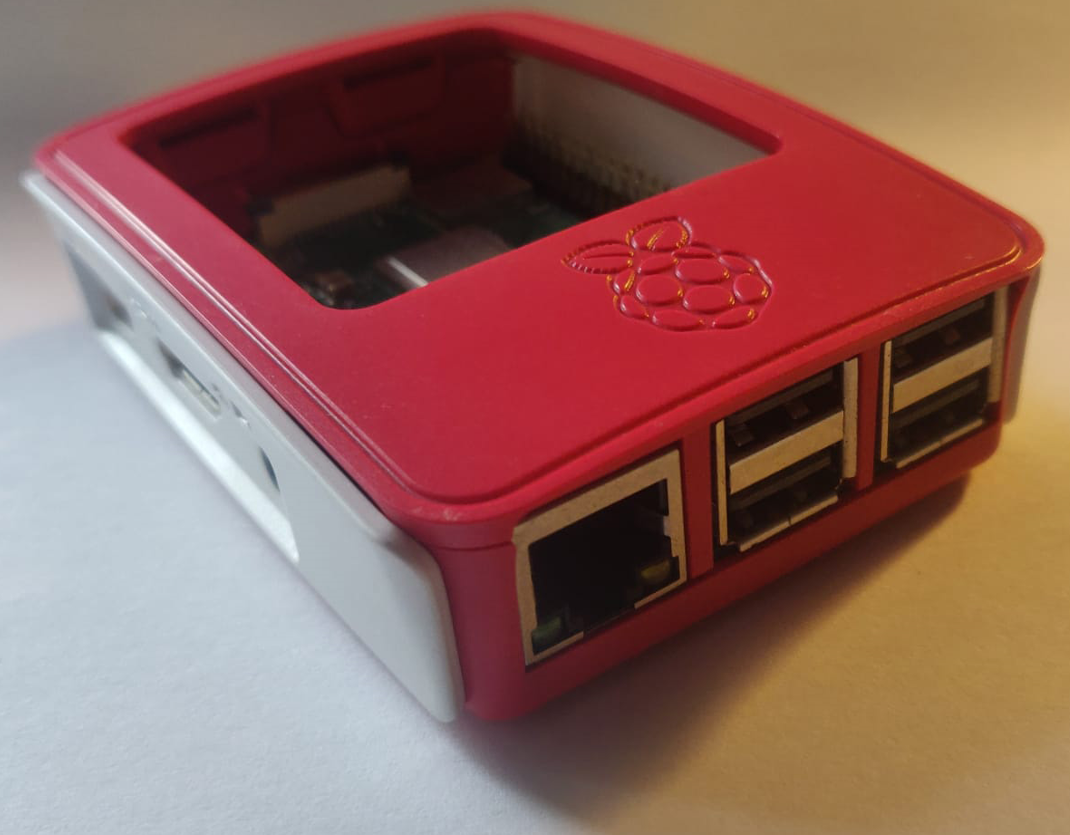
\includegraphics[height=250pt]{pi_mitgehaeuse.png}
	\caption{Raspberry Pi 3B+}
	\label{pi_mitgehaeuse}
\end{figure}	

\subsubsection{Raspberry Pi für das Projekt}
Für das Projekt Überwachungssystem mittels der IMU des M5 Sticks soll ein 
Raspberry Pi 3B+ als sogenannter IoT Broker und als Aktor für den Alarm genutzt werden.\par
%Das Modell 3B+ verfügt über eine Rechenleistung von
Der Raspberry Pi 3B+ wurde für das Projekt am besten geeignet eingestuft. Er verfügt über einen Gigabit-LAN Anschluss welcher mit Hilfe eines Ethernetkabels für eine stabile Verbindung mit dem Router des Heimnetzwerkes sorgen soll. Verglichen mit älteren Raspberry Pi Modellen ist der 3B+ mit einer etwas stärkeren CPU, sowie einer WLAN und Bluetooth Karte ausgestattet, welche die Möglichkeiten bieten das Projekt um mehr IoT Geräte, beispielsweise Sensoren und Aktoren, zu erweitern. Zudem ist der preisliche Unterschied (UVP) zu den Vorgängermodellen marginal.  

	\begin{figure}[H]
	\centering
	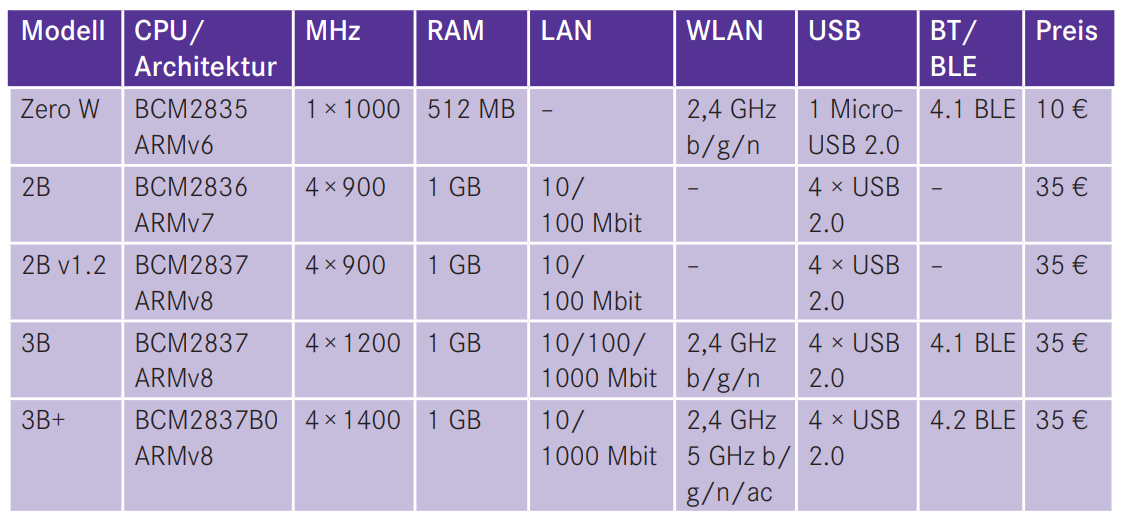
\includegraphics[height=200pt]{tabelle_pi_vergleich}
	\caption{Vergleich der verschiedenen Raspberry Pi Modelle \protect\cite[S. 59]{Huwe.2019}}
	\label{tabelle_pi_vergleich}
\end{figure}

\subsubsection{Anschlussmöglichkeiten am Raspberry Pi 3B+}
Der Raspberry Pi 3B+ verfügt im Allgemeinen über folgende Anschlussmöglichkeiten (siehe Abb. \ref{RaspiAnschluesse}):\footnote{\cite[S. 60]{Huwe.2019}}\par 
$\bullet$ HDMI   \par %\hspace{20pt} $\bullet$ 
$\bullet$ 3,5mm AUX\par 
$\bullet$ 4 $\times$ USB 2.0 \par 
$\bullet$ Ethernet 1Gbit/RJ45\par 
$\bullet$ CCI (Camera Connector Interface)\par 
$\bullet$ DSI (Display Serial Interface)\par
$\bullet$ 40 GPIO-Pins\par
$\bullet$ Steckplatz für die microSD-Karte\par
$\bullet$ Micro-USB Anschluss für die Stromversorgung des PIs\par

	\begin{figure}[H]
		\centering
		\includegraphics[width=15cm]{RaspiAnschluesse}
		\caption{Hardwarebezeichnung auf Pi mit Beschriftung \cite{.06.03.2019}}
		\label{RaspiAnschluesse}
	\end{figure}
	
Für das Projekt sind insbesondere die GPIO-Pins und der Ethernetport von Bedeutung.\par

\newpage

\subsection{Weitere Hardware}
\subsubsection{Piezo Buzzer Modul}
	Um beim Auslösen der Alarmanlage ein Warnsignal zu erzeugen, soll ein aktives Piezo Buzzer Modul ST1143 der Marke Iduino (Abb. \ref{ST1143}) eingesetzt werden.\par Die Pins des Buzzers werden wie folgt mittels Jumperkabeln mit den GPIO Pins des Pis verbunden (Tab. \ref{BuzzerTabelle}, Abb. \ref{BuzzerAnschluss}): \footnote{\cite{Draeger.2019}}
	
	\begin{table}[H]
		\centering
		\begin{tabular}{|p{5cm}|p{5cm}|} 
			\hline
			Buzzer & Raspberry Pi\\ 
			\hline
			SIG (S)   & GPIO 4 \hspace{0,1cm}(Pin 7)\\  
			\hline
			VCC~ ($+$; mittlerer Pin)   & 3,3V 	\hspace{0,7cm}(Pin 1)\\
			\hline
			GND (-)    & Ground  	\hspace{0,2cm}(Pin 6)\\
			\hline
		\end{tabular}
	\caption{Verbindung ST1143 mit Pi}
	\label{BuzzerTabelle}
	\end{table} 

	\begin{figure}[H]
	\centering
	\includegraphics[width=10cm]{BuzzerAnschluss}
	\caption{Schaltplan ST1143 an Raspberry Pi}
	\label{BuzzerAnschluss}
	\end{figure}

	\begin{figure}[H]	%H
	\centering
	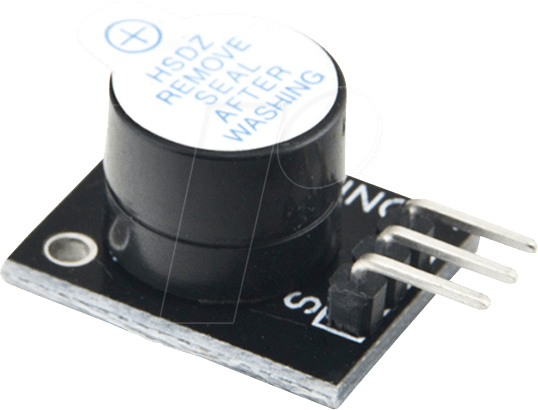
\includegraphics[height=150pt]{ST1143}
	\caption{Aktiver Piezo Buzzer ST1143 \cite{reicheltelektronikGmbH&amp.21.04.2022}}
	\label{ST1143}
	\end{figure}

\subsubsection{Taster}

Der Alarm soll über ein Tastermodul SBC-BUTTON2 (Abb. \ref{BUTTON2}) mit jeweils einem Button deaktiviert beziehungsweise manuell aktiviert werden können.
Das Modul wird mittels Jumperkabeln mit den GPIO Pins des Pis verbunden (siehe Schaltplan Abb. \ref{TasterAnschluss} und Tabelle \ref{TasterTabelle}). 
In der gewählten Anschlusskonfiguration wird das Modul als High-Aktiv betrieben. Dies bedeutet, dass bei Tastendruck der GPIO23 bzw. GPIO24 mit der Spannungsquelle verbunden wird und der Raspberry PI jeweils ein HIGH Signal erhält. \footnote{\cite{.19.04.2022}}\par 
Es wäre ebenfalls möglich durch vertauschen des VCC und GND Anschlusses das Modul als Low-Aktiv zu betreiben.

\begin{table}[H]
	\centering
	\begin{tabular}{|p{5cm}|p{5cm}|} 
		\hline
		Tastermodul & Raspberry Pi\\ 
		\hline
		SIG(S1)                   & GPIO 23 \hspace{0,3cm}(Pin 16)\\
		\hline
		SIG(S2)                   & GPIO 24 \hspace{0,3cm}(Pin 18)\\
		\hline
		VCC~(+)   & 5V \hspace{1,45cm}(Pin\hspace{0,35cm}4)\\ 
		\hline
		GND(-)                   & Ground \hspace{0,6cm}(Pin 14)\\
		\hline
		
\end{tabular}
	\caption{Verbindung Taster SE043 mit Pi}
	\label{TasterTabelle}
\end{table}

	\begin{figure}[H]
	\centering
	\includegraphics[width=15cm]{TasterAnschluss}
	\caption{Schaltplan Taster SE043 an Raspberry Pi}
	\label{TasterAnschluss}
	\end{figure}

	\begin{figure}[h] %H
	\centering
	\includegraphics[height=150pt]{BUTTON2}
	\caption{Joy-it SBC-BUTTON2 \cite{reicheltelektronikGmbH&amp.21.04.2022b}}
	\label{BUTTON2}
	\end{figure}

\subsubsection{Zubehör des Raspberry Pi}
Für die Spannungsversorgung soll ein originales Raspberry Pi Micro-USB-Netzteil mit einer maximal abrufbaren Leistung von 13W genutzt werden.\par

Eine MicroSDHC-Speicherkarte mit einer Kapazität von 16GB und einer Lesegeschwindigkeit von bis zu 90 MB/s soll den nötigen Speicher für den Mosquitto MQTT Broker und weitere Aufgaben bereitstellen. \href{\linkmicrosd}{(Reichelt Bestelllink)} 

\newpage

\subsection{Anschlussplan Raspberry Pi}
Der Anschluss der Hardwarebauteile an den Pi erfolgt über die auf dem Pi verbauten Pins laut Anschlussplan (Abb. \ref{Anschlussplan}). Der Raspberry Pi benötigt einen Anschluss per Micro-USB zur Spannungsversorgung. Dies kann, je nach Anliegen, entweder über den Router erfolgen, sofern dieser über eine USB-Schnittstelle verfügt, oder über einen externen Spannungswandler (vgl. Handyladegerät). Der Warnsummer/Buzzer benötigt keine externe Spannungsquelle und wird direkt über den Pi mit Spannung versorgt.

\begin{figure}[H]	%[H] um an dieser Stelle anzuzeigen
\begin{center}
\includegraphics[width=15cm]{Anschlussplan.png}
\caption{Anschlussschematik Raspberry Pi 3}
\label{Anschlussplan}
\end{center}
\end{figure}

\newpage

\section{Verzeichnisse}
\addcontentsline{toc}{subsection}{Abbildungsverzeichnis}
\listoffigures %Abbildungsverzeichnis
\addcontentsline{toc}{subsection}{Tabellenverzeichnis}
\listoftables
\addcontentsline{toc}{subsection}{Literatur}
\bibliography{Literatur}	%Literaturverzeichnis

\end{document}
